\documentclass{article}
\usepackage[margin=1cm]{geometry}
\usepackage{setspace}
\usepackage{listings}
\usepackage{xcolor}
\usepackage{multicol}
\usepackage{amsmath}
\geometry{left=1in,right=1in,top=1in,bottom=1in}

\usepackage{subcaption} % i used this for the 2B part in 2B3 only in MPEG 

% Set the basic style to a coding-style font
\definecolor{lightyellow}{RGB}{255, 255, 224}
\definecolor{lightgreen}{RGB}{144,238,144}
\definecolor{darkgreen}{RGB}{0,128,0}

\lstset{
    backgroundcolor=\color{lightyellow},
    basicstyle=\color{darkgreen}\fontsize{10}{12}\ttfamily,
    frame=single,
    breaklines=true,
    columns=fullflexible,
    xleftmargin=0.05 in,
    xrightmargin=0.05in
}

% Importing your images here. Don't put it inside the document class
\usepackage{graphicx}
	\graphicspath{ {./imgs/} }

% Define title page
\newcommand{\mytitlepage}{
    \begin{titlepage}
        \begin{center}
            \vspace*{1.5cm}
            
            \LARGE\textbf{ASSIGNMENT 2}
            \vspace{0.5cm}\\
            \Large CMSC 178\\
            \Large Digital Image Processing\\
            \vspace{3cm}
            Submitted to:\\
            Mr. Dhong-Fhel K. Gom-os\\
            
            \vspace{2.5cm}
            Submitted by:\\
            Lyka Jeanine L. Panchacala\\
            Wineff Chen Zhen Y. Gulane
            
            \vspace{4cm}
            
	April 2023
            
            \vspace{1.3cm}
        \end{center}
        \large\textbf{Overview}\\
        The assignment was aimed at providing a practical learning opportunity in digital image manipulation using MATLAB, while also reinforcing our knowledge of the foundational concepts in image processing covered in the course. As part of the task, we were required to modify various functions to carry out basic yet essential techniques such as color correction, contrast enhancement, and noise filtering. The main objective was to acquire hands-on experience with these methods.
    \end{titlepage}
}

\begin{document}

	\mytitlepage

	\newpage
	\section*{Exercise 2A –  ( 5\% ) – De-convolution using a Wiener Filter}
	
	\subsection*{1. Background of the Problem}
	Color balancing is a critical aspect of image processing, but achieving accurate color balance can be challenging, especially when working with images captured under non-standard lighting conditions or different cameras or devices. One approach to color balancing is to use a reference chart, and in this exercise, three simple functions are required:
	\begin{itemize}
	\item {\texttt{get\textunderscore chart\textunderscore values.m}} – extracts samples from the 24-color chart image; and 
	\item {\texttt{chart\textunderscore correct.m}}  – calculates the mapping between the ideal and less than ideal cases using the extracted values from both charts. 
	\item {\texttt{apply\textunderscore rgb\textunderscore map.m}} –  applies this mapping to an image to correct for color imbalance.
	\end{itemize}
 These functions can be useful in various applications that require accurate color representation, such as photography, graphic design, and other fields where visual content is critical.
 AAA
 AAA

 AAA

 AAA
 AAA
 AAA
 
 AAA
 AAA
 AAA
 AAA
 AAA
 AAA
 AAA
 AAA
 AAA
 AAA
 AAA
 AAA
 AAA
 AAA
 AAA
 





	\subsection*{2. Procedure}
	We used the {\texttt{wiener\_deblur.m}} function for image deblurring using the Wiener deconvolution algorithm. This function is already supplied however it is incomplete and cannot be used. 
	We need to modify the {\texttt{wiener\_deblur.m}} function to implement the algorithmic process of Wiener Deconvolution. Inside the {\texttt{wiener\_deblur.m}} function, these following 
	functions are used: {\texttt{floor()}}, {\texttt{padarray()}}, {\texttt{zeros()}}, {\texttt{abs()}}, {\texttt{ifft2()}}, {\texttt{real()}}, and {\texttt{ifftshift()}}. 
	The remaining functions, {\texttt{edgetaper()}} and {\texttt{fft2()}}, are already supplied. The {\texttt{floor}} function is used to get the floor values of the padding size. 
	The {\texttt{padarray}} function is used to pad zeros to the blur kernel. 
	The {\texttt{zeros}} function is used to instantiate an array of zeros. 
	The {\texttt{absolute}} function is used to ensure that only magnitude is used for the inverse filter. 
	The {\texttt{inverse fast fourier transformation 2}} function is used to convert an image from spatial domain to the frequency domain. 
	The {\texttt{real}} function is used to extract the real values used for the final deblurred image. 
	And the {\texttt{inverse fast fourier transform shift}} or {\texttt{inverse zero-frequency shift}} is used to shift the zero-frequency component of the DFT to the center of the array 
	effectively shifting the image back to its original position putting the image back in the top-left corner.
	
	The algorithm Wiener deconvolution is used to remove the blurriness from an image caused by a known blur kernel. The code modifications we have added focuses on the main steps through using 
	zero padding, inverse filtering, image reconstruction, and spatial delay handling. The first step is to add zero padding. To begin, the initial step involves applying zero padding to the blur kernel. 
	This adjustment ensures that the kernel matches the size of the input image. This serves the purpose of convenient element-wise multiplication in the frequency domain. 
	Although, Wiener deconvolution does not require zero padding, this step simply adds ease or convenience when dealing with the next steps. We then compute for the Fast Fourier Transform 
	representation of the blur kernel. Next step is to compute wiener inverse filter through this formula:
	\[F_{\text{inv}} = \frac{F_I}{F_B} \frac{|F_b|^2}{|F_B|^2 + k}\]
	the {\texttt{$F_{inv}$}} can then be calcuated through element-wise multiplication and division in {\texttt{MATLAB}}. Other way of solving this is to iterate each pixels and calculate their values.
	But using element-wise operation is much more efficient in vector operations compared to iterating in loops. The next step is to convert the image back to the frequency domain from the spatial domain
	and then acquire its real values that will be used to display the image. The reason why real values are extracted is because complex numbers in the Wiener inverse filter may include 
	negative and imaginary values, but in the frequency domain, negative values are not utilized as the focus is typically on magnitude and phase information. Displaying the complex numbers would
	probably alter the image however testing the image example in this exercise did not alter much of the image and still looked similar with real values being extracted. Once the wiener inverse filter
	is calculated and extracted for display, the last step is to fix the spatial delays or zero values due to the zero padding.





	\subsection*{3. Results and Discussion}
	In this section, we present the outcomes of our modified {\texttt{wiener blur}} function and analyze how the outputs are influenced by the selected parameters or configurations. 
	The sample image inputs we used are already provided from this laboratory exercise and their corresponding outputs are showcased to demonstrate the function's behavior. There are a total of three (3)
	tests for {\texttt{deconv\_test.m}} function with varying parameters: {\texttt{K=0.01}}, {\texttt{K=0.9}}, and {\texttt{K=0.000001}}. The following figures below are the original image inputs:
	\begin{figure*}[ht]
  	\centering
  	\begin{minipage}[t]{0.45\textwidth}
    	\centering
    	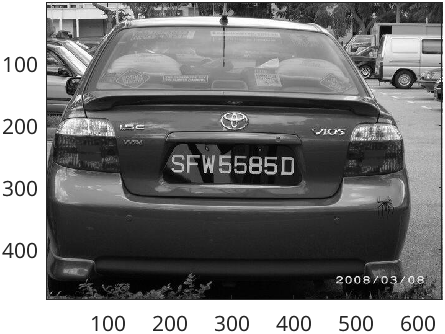
\includegraphics[width=\textwidth]{2AE1Orig}
    	\caption{Sample Input Image 1}
    	\label{fig:example1}
  	\end{minipage}\hfill
  	\begin{minipage}[t]{0.45\textwidth}
    	\centering
    	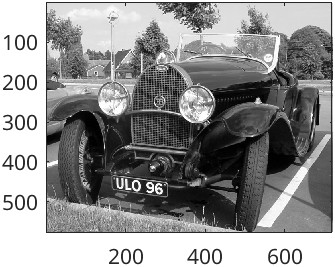
\includegraphics[width=\textwidth]{2AE2Orig}
    	\caption{Sample Input Image 2}
    	\label{fig:example2}
  	\end{minipage}
	\end{figure*}

	Since only the parameter K value has been changed, these figures below will be used as the default corrupted data of the two input images:
	\begin{figure*}[ht]
  	\centering
  	\begin{minipage}[t]{0.45\textwidth}
    	\centering
    	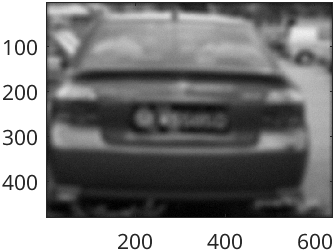
\includegraphics[width=\textwidth]{2AE1Corrupted}
    	\caption{Corrupted Data of Input Image 1}
    	\label{fig:example1corrupted}
  	\end{minipage}\hfill
  	\begin{minipage}[t]{0.45\textwidth}
    	\centering
    	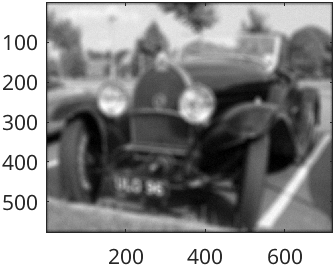
\includegraphics[width=\textwidth]{2AE2Corrupted}
    	\caption{Corrupted Data of Input Image 2}
    	\label{fig:example2corrupted}
  	\end{minipage}
	\end{figure*}


	The following below are the tests cases:
	\begin{itemize}
  	\item \textbf{Parameter K = 0.01} – This test only modifies the K parameter value to 0.01 which is the default parameter K from the exercise.

			\begin{figure}[ht]
  			\centering
  			\begin{minipage}[t]{0.40\textwidth}
    			\centering
    			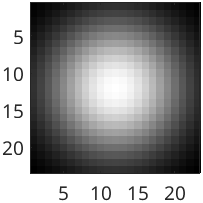
\includegraphics[width=\textwidth]{2AE1PSF}
    			\caption{PSF of Sample Input Image 1}
    			\label{fig:psf1}
  			\end{minipage}\hfill
  			\begin{minipage}[t]{0.40\textwidth}
    			\centering
    			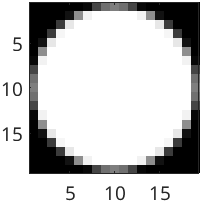
\includegraphics[width=\textwidth]{2AE2PSF}
    			\caption{PSF of Sample Input Image 2}
    			\label{fig:psf2}
  			\end{minipage}
			\end{figure}

			Figure {\ref{fig:psf1}} and Figure {\ref{fig:psf2}} are the guessed PSF values used for deblurring the image. 

			\begin{figure}[ht]
  			\centering
  			\begin{minipage}[t]{0.40\textwidth}
    			\centering
    			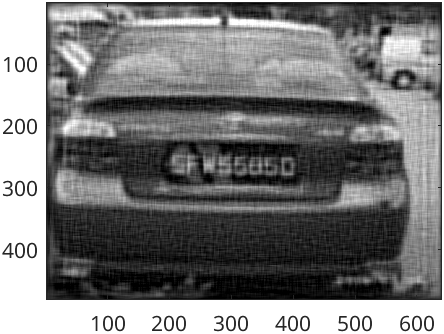
\includegraphics[width=\textwidth]{2AE1K0.01}
    			\caption{Deconvuled of Sample Input Image 1}
    			\label{fig:deblur1}
  			\end{minipage}\hfill
  			\begin{minipage}[t]{0.40\textwidth}
    			\centering
    			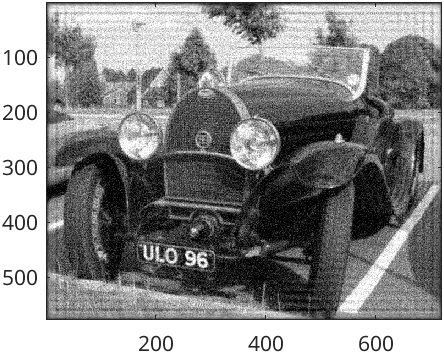
\includegraphics[width=\textwidth]{2AE2K0.01}
    			\caption{Deconvuled of Sample Input Image 2}
    			\label{fig:deblur2}
  			\end{minipage}
			\end{figure}

			Based on these two images Figure {\ref{fig:deblur1}} and Figure {\ref{fig:deblur2}}, the license plate numbers can be clearly seen but as you can see there are a bit of blocks pattern
			on the image. But for Figure {\ref{fig:deblur1}}, the license plate number is a bit harder to read. Thus, we have tested Figure {\ref{fig:example1}} with K value of {\texttt{0.001}}.
			
			\begin{figure}[ht]
  			\begin{minipage}{0.4\textwidth}
    			\centering
    			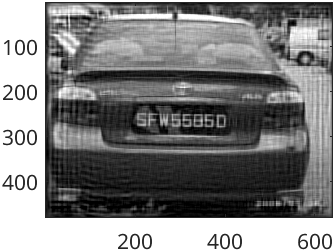
\includegraphics[width=\textwidth]{2AE1K0.001}
    			\caption{Deconvolution of Sample Input Image 1 at K=0.001}
    			\label{fig:deblur1a}
  			\end{minipage}
  			\hfill
  			\begin{minipage}{0.35\textwidth}
    			The license plate number in Figure {\ref{fig:deblur1a}} is now much clearer compared to the image with {\texttt{K=0.01}}.
  			\end{minipage}
			\end{figure}

			The results shows that the deconvoled output figures of the sample input images will have different parameter K values and their PSF can differ depending on the images. We have tested
			both K values for the same images but in order to depict the image with clarity, we further tested {\ref{fig:example1}} with another K value. The result was far clearer in comparison
			with the default K value. Basing on this test case result, we decided to further test on checking the result of a higher parameter K.


  	\item \textbf{Parameter K = 0.9} – In this test, we tried to acquire the result of the deconvoled image if K is {\texttt{0.9}}.

  		\begin{figure}[ht]
  			\centering
  			\begin{minipage}[t]{0.45\textwidth}
    			\centering
    			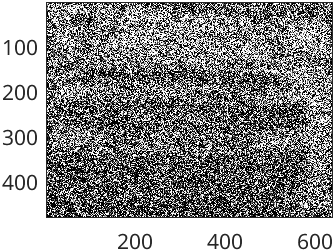
\includegraphics[width=\textwidth]{2AE1Corrupted2}
    			\caption{Corrupted Data of Sample Input Image 1}
    			\label{fig:corrupted_e1}
  			\end{minipage}\hfill
  			\begin{minipage}[t]{0.45\textwidth}
    			\centering
    			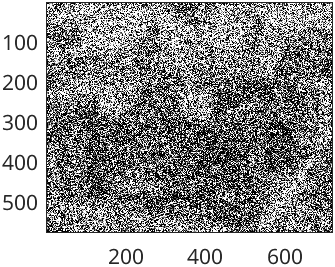
\includegraphics[width=\textwidth]{2AE2Corrupted2}
    			\caption{Corrupted Data of Sample Input Image 2}
    			\label{fig:corrupted_e2}
  			\end{minipage}
			\end{figure}

			To much of our surprise, {Figure~\ref{fig:corrupted_e1}} and {Figure~\ref{fig:corrupted_e2}} has changed. We did not expect that changing the parameter K value would alter the result of
			the corrupted image. As it turns out, modifying {\texttt{K}} was actually the noise standard deviation which may also be the blur kernel.

  		\begin{figure}[ht]
  			\centering
  			\begin{minipage}[t]{0.45\textwidth}
    			\centering
    			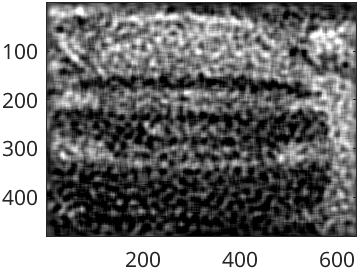
\includegraphics[width=\textwidth]{2AE1K0.9}
    			\caption{Deconvuled Sample Input Image 1}
    			\label{fig:deconv_e1_2}
  			\end{minipage}\hfill
  			\begin{minipage}[t]{0.45\textwidth}
    			\centering
    			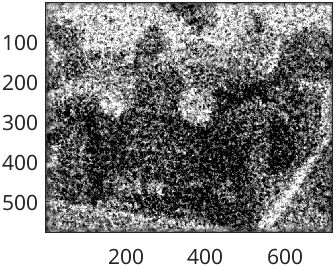
\includegraphics[width=\textwidth]{2AE2K0.9}
    			\caption{Deconvuled Sample Input Image 2}
    			\label{fig:deconv_e2_2}
  			\end{minipage}
			\end{figure}

			{Figure~\ref{fig:deconv_e1_2}} and {Figure~\ref{fig:deconv_e2_2}} exhibits noticeable degradation in terms of clarity. Due to the presence of extensive image noise, only a limited portion of the image quality was successfully restored using 
			our wiener deblur function. The substantial loss of data caused by the noise renders a complete recovery of the image impossible.


		\item \textbf{Parameter K = 0.000001} – In this test, we tried to acquire the result of the deconvoled image if K is {\texttt{0.000001}}.

  		\begin{figure}[ht]
  			\centering
  			\begin{minipage}[t]{0.45\textwidth}
    			\centering
    			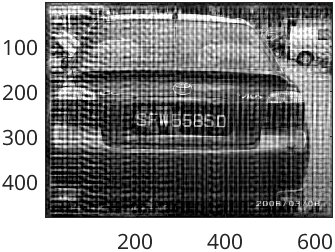
\includegraphics[width=\textwidth]{2AE1K0.000001}
    			\caption{Deconvoled Sample Input Image 1}
    			\label{fig:deconv_e1_3}
  			\end{minipage}\hfill
  			\begin{minipage}[t]{0.45\textwidth}
    			\centering
    			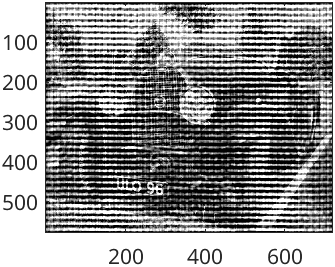
\includegraphics[width=\textwidth]{2AE2K0.000001}
    			\caption{Deconvoled Sample Input Image 2}
    			\label{fig:deconv_e2_3}
  			\end{minipage}
			\end{figure}

			{Figure~\ref{fig:deconv_e1_3}} and {Figure~\ref{fig:deconv_e2_3}} demonstrate minimal noticeable noise, closely resembling Figures {Figure~\ref{fig:example1corrupted}} and 
			{Figure~\ref{fig:example2corrupted}}, which represent the corresponding corrupted data. However, upon closer examination of the output images, line-like artifacts are apparent along the 
			X and Y axes. These artifacts indicate the challenges faced by our wiener deblur function in effectively restoring the image to its original clarity.

		\item \textbf{Parameter K = 0.01 (without deblurring)} – In this test, similar parameter K value is used to the first test however we do not blur the image.

  		\begin{figure}[ht]
  			\centering
  			\begin{minipage}[t]{0.45\textwidth}
    			\centering
    			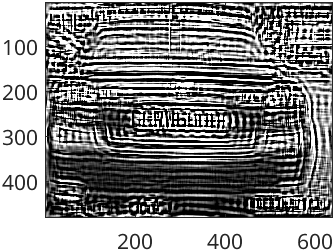
\includegraphics[width=\textwidth]{2AE1NoBlur}
    			\caption{Deconvoled Sample Input Image 1}
    			\label{fig:deconv_e1_4}
  			\end{minipage}\hfill
  			\begin{minipage}[t]{0.45\textwidth}
    			\centering
    			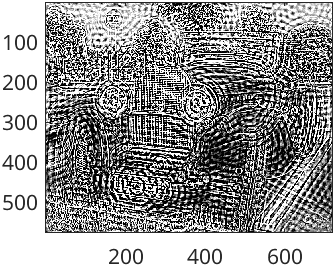
\includegraphics[width=\textwidth]{2AE2NoBlur}
    			\caption{Deconvoled Sample Input Image 2}
    			\label{fig:deconv_e2_4}
  			\end{minipage}
			\end{figure}

			{Figure~\ref{fig:deconv_e1_4}} and {Figure~\ref{fig:deconv_e2_4}} skips the blurring process and directly undergo to the deblurring process. The output images do not resemble 
			the input images but instead they exhibit distortions resembling the visual effects associated with LSD usage.

		\item \textbf{Parameter K = 0.01 (laplacian and sobel blur filter)} – In this test, similar parameter K value is used to the first test however we have changed the blur filter being used for the input images.

  		\begin{figure}[ht]
  			\centering
  			\begin{minipage}[t]{0.45\textwidth}
    			\centering
    			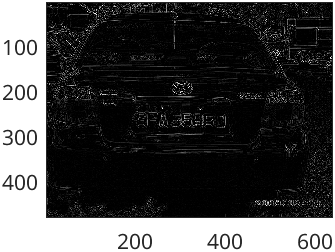
\includegraphics[width=\textwidth]{2AE1Corrupted_laplacian}
    			\caption{Corrupted Data of Sample Input Image 1}
    			\label{fig:laplacian_cd}
  			\end{minipage}\hfill
  			\begin{minipage}[t]{0.45\textwidth}
    			\centering
    			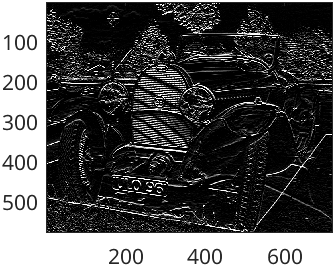
\includegraphics[width=\textwidth]{2AE2Corrupted_sobel}
    			\caption{Corrupted Data of Sample Input Image 2}
    			\label{fig:sobel_cd}
  			\end{minipage}
			\end{figure}

  		\begin{figure}[ht]
  			\centering
  			\begin{minipage}[t]{0.45\textwidth}
    			\centering
    			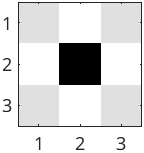
\includegraphics[width=\textwidth]{2AE1PSF_laplacian}
    			\caption{PSF of Sample Input Image 1}
    			\label{fig:laplacian_psf}
  			\end{minipage}\hfill
  			\begin{minipage}[t]{0.45\textwidth}
    			\centering
    			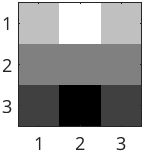
\includegraphics[width=\textwidth]{2AE2PSF_sobel}
    			\caption{PSF of Sample Input Image 2}
    			\label{fig:sobel_psf}
  			\end{minipage}
			\end{figure}

  		\begin{figure}[ht]
  			\centering
  			\begin{minipage}[t]{0.45\textwidth}
    			\centering
    			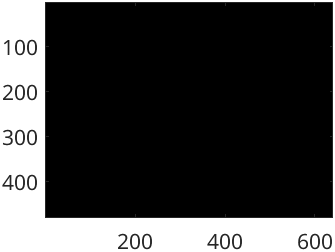
\includegraphics[width=\textwidth]{2AE1K0.01_laplacian}
    			\caption{Deconvoled Sample Input Image 1}
    			\label{fig:laplacian_decon}
  			\end{minipage}\hfill
  			\begin{minipage}[t]{0.45\textwidth}
    			\centering
    			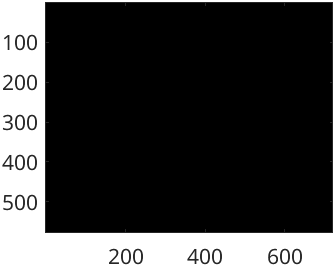
\includegraphics[width=\textwidth]{2AE2K0.01_sobel}
    			\caption{Deconvoled Sample Input Image 2}
    			\label{fig:sobel_decon}
  			\end{minipage}
			\end{figure}

			We applied different blur filters to the images: Laplacian blur filter in Figure~\ref{fig:laplacian_cd} and Sobel filter in Figure~\ref{fig:sobel_cd}. 
			The purpose of using these filters was to observe their effect on the images and compare it with the Gaussian filter. As shown in the figures, it is evident that a 
			significant amount of details has been lost due to the blurring process. The blurring caused a considerable degradation in the image quality, making the recovery of the original 
			image nearly impossible unlike Gaussian filter.

			As a proof to that statement, we present Figure~\ref{fig:laplacian_decon} and Figure~\ref{fig:sobel_decon}. These figures show the deconvolution results after applying the 
			Wiener deblur algorithm to the blurred images. Despite the attempt to deblur the images, the resulting outputs still exhibit substantial artifacts and the images being black. 
			These artifacts are remnants of the severe degradation introduced by Laplacian and Sobel filters.

	\end{itemize}
	
	\vspace{15pt}
	\noindent{\textbf{Deblurring Six Plate Numbers}}
	\par
	\vspace{10pt}
	In order to further test our implemented function, we tested this against six plate numbers that have been blurred. It is assumed that Gaussian filtered was applied. Our goal for this
	test is to guess which {\texttt{K}} parameter value works best in deblurring the plate numbers. {Figure~\ref{fig:2AE3_Blurred}} shows the blurred plate numbers that needs to be deblurred
	using our implemented wiener deconvolution function and {Figure~\ref{fig:2AE3_PSF}} is the PSF guess. We tested guessing {\texttt{K}} at {\texttt{0.01}}, {\texttt{0.001}}, 
	{\texttt{0.003}}, and {\texttt{0.005}}.

	Based on our test results, the parameter with the value of {\texttt{K}} would be {\texttt{0.003}} since all the six plate numbers can be read. These six numbers are: {\texttt{EN 1113}}, {\texttt{DT 1735}}, 
	{\texttt{CD 7984}}, {\texttt{BT 9824}}, {\texttt{WYG 734}}, and {\texttt{IT 0420}}.

  	
	\begin{figure}[ht]
  	\centering
  	\begin{minipage}[t]{0.45\textwidth}
    	\centering
    	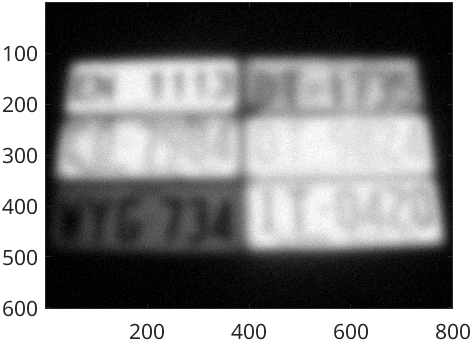
\includegraphics[width=\textwidth]{2AE3_Blurred}
    	\caption{Blurred Six Plate Numbers}
    	\label{fig:2AE3_Blurred}
  	\end{minipage}\hfill
  	\begin{minipage}[t]{0.45\textwidth}
    	\centering
    	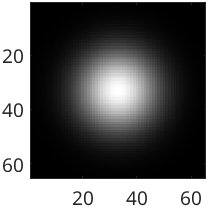
\includegraphics[width=\textwidth]{2AE3_PSF}
    	\caption{PSF Guess for Six Plate Numbers}
    	\label{fig:2AE3_PSF}
  	\end{minipage}
	\end{figure}


	\begin{figure}[ht]
  	\centering
  	\begin{minipage}[t]{0.45\textwidth}
    	\centering
    	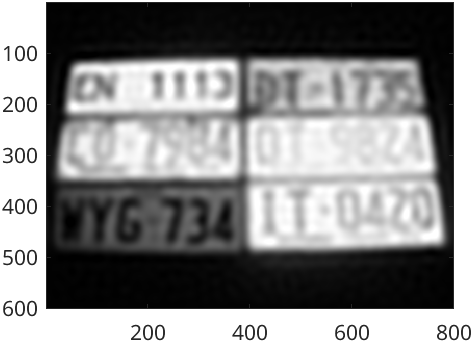
\includegraphics[width=\textwidth]{2AE3_D01}
    	\caption{K = 0.01}
    	\label{fig:2AE3_D01}
  	\end{minipage}\hfill
  	\begin{minipage}[t]{0.45\textwidth}
    	\centering
    	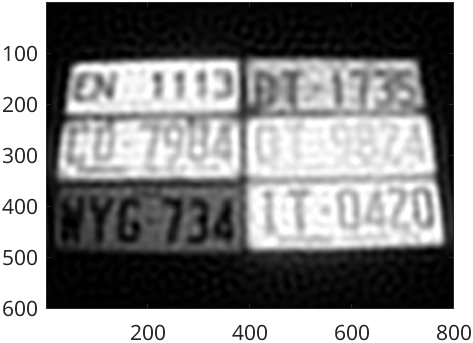
\includegraphics[width=\textwidth]{2AE3_D001}
    	\caption{K = 0.001}
    	\label{fig:2AE3_D001}
  	\end{minipage}
	\end{figure}


	\begin{figure}[ht]
  	\centering
  	\begin{minipage}[t]{0.45\textwidth}
    	\centering
    	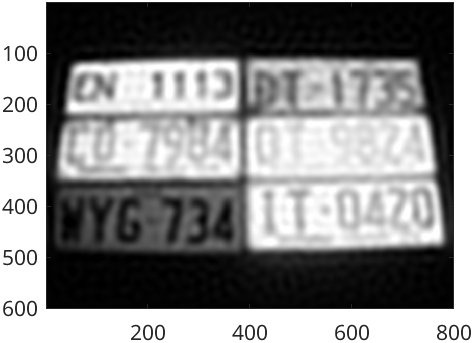
\includegraphics[width=\textwidth]{2AE3_D003}
    	\caption{K = 0.003}
    	\label{fig:2AE3_D003}
  	\end{minipage}\hfill
  	\begin{minipage}[t]{0.45\textwidth}
    	\centering
    	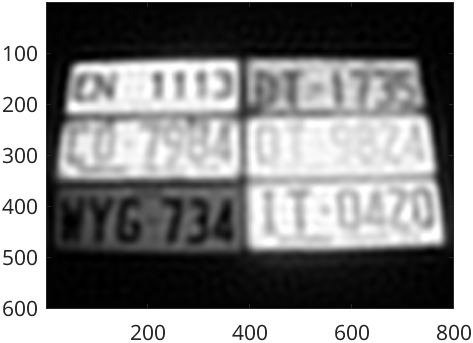
\includegraphics[width=\textwidth]{2AE3_D005}
    	\caption{K = 0.005}
    	\label{fig:2AE3_D005}
  	\end{minipage}
	\end{figure}




	\par\vspace{10pt}

	Overall, these sample test cases highlight the expected output of our modified wiener blur function similarly to the laboratory exercise's outputs. The variation of the parameter K has a 
	significant impact on both the corrupted data and the deconvolved image. When the K value approaches 1, excessive noise becomes evident in the output. Conversely, selecting a K value 
	close to 0 minimizes the presence of noise, but introduces line-like artifacts in the resulting image. It is important to note that deblurring the image is a necessary prerequisite for 
	the proper functioning of the Wiener Deconvolution algorithm.

	\clearpage





	\subsection*{4. Comments and Conclusion}
	The {\texttt{wiener\_deblur.m}} function is implemented to deblur an input image using the Wiener deconvolution algorithm. The optimal output can be achieved by selecting suitable parameters or 
	configurations. The key parameter in this function is the regularization parameter {\texttt{K}}. Adjusting the value of {\texttt{K}} allows controlling the trade-off between noise reduction 
	and clarity of the deblurred image. Generally, a smaller value of {\texttt{K}} results in less noise but may introduce artifacts or line-like distortions in the output. On the other hand, 
	a larger value of {\texttt{K}} would result in an increased noise standard deviation, leading to higher levels of noise in the output image. There is no best parameter or configurations since
	it would depend on the blurr level intensity of the input image. Experimenting the values for different images would be the best result.

	One limitation of the our modified function is that it assumes the blurring model being used, such as a Gaussian blur kernel. While it may work well for images blurred by this model, 
	it may not be as effective for images blurred using different kernels or complex blurring mechanisms which is evident in our Results and Discussions. 



	\vspace{0.5cm}
	
	\newpage
	\section*{Exercise 2B –  ( 5\% ) – Motion Image Compression}
	
	\subsection*{1. Background of the Problem}


	\subsection*{2. Procedure}
	There are two functions, {\texttt{jpeg\_8x8.m}} and {\texttt{simple\_mpeg.m}}, that are supplied from this laboratory exercise as a guide to modify two incomplete functions, 
	{\texttt{djpeg\_8x8.m}} and {\texttt{simple\_dmpeg.m}}, that effectively decode an image and a video. We first focused on {\texttt{djpeg\_8x8.m}} that implements the decoding 
	process for the image. It first copies the DC coefficient to the quantized coefficient array. The first and second element or index in the array is the DC while the rest 
	are the AC coefficients. Which is to be used for iterating the array in zig-zag pattern where the AC coefficient index is assigned to the quantized array while ensuring 
	the direction. Where its next step is to acquire its quantization scale factor to determine the level of compression applied to the coefficients in the array. We then 
	perform the inverse quantization step in the JPEG decoding process. It reconstructs the original DCT coefficients from the quantized coefficients by applying the 
	quantization table and the Q scale factor. The result would be then a matrix that represents a reconstructed DCT coefficients which will be used for IDCT. In the final step, 
	we use the inverse discrete cosine transform to convert the frequency coefficients back into pixel values. This process, performed with the help of the idct() function from the 
	signal processing toolbox, allows us to reconstruct the 8x8 image block tile to its original form.

	After performing the decoding process for images, the next step of the laboratory exercise is to implement the decoding of MPEG video formats. We modified {\texttt{simple\_dmpeg.m}}
	to iterate over the 8x8 block in an image. Two frames are compared to each other and analyzed to see whether there is a change in pixels. Blocks that had similar coefficient values
	are ignored and blocks that do have differences are extracted. The intention of this function is not to iterate over each frames in the video but instead to compare two frames. 
	It is the job of {\texttt{mpeg\_test.m}} to iterate each frames. Once the decompression of the frame is done, an output is generated.




	\subsection*{3. Results and Discussion}

	In this section, we show the results of {\texttt{djpeg\_8x8.m}} and {\texttt{simple\_dmpeg.m}} and analyze its outputs based on given parameter configurations. Sample input images are
	already provided. Using {Figure~\ref{fig:2B_Input}} and {Figure~\ref{fig:2B_Input2}} as inputs, we where able to acquire its decompressed image 
	shown on {Figure~\ref{fig:2B_Decom1}} and {Figure~\ref{fig:2B_Decom2}}. Their difference is shown on {Figure~\ref{fig:2B_Diff1}} and {Figure~\ref{fig:2B_Diff2}}.


	\begin{figure}[ht]
  	\centering
  	\begin{minipage}[t]{0.45\textwidth}
    	\centering
    	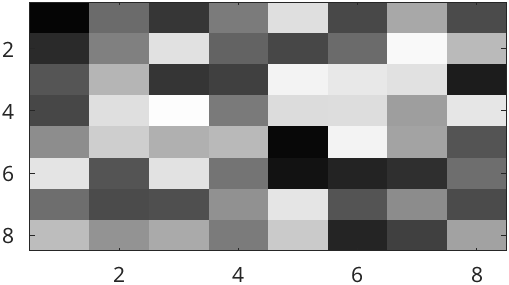
\includegraphics[width=\textwidth]{2B_Input}
    	\caption{JPEG Input 1}
    	\label{fig:2B_Input}
  	\end{minipage}\hfill
  	\begin{minipage}[t]{0.45\textwidth}
    	\centering
    	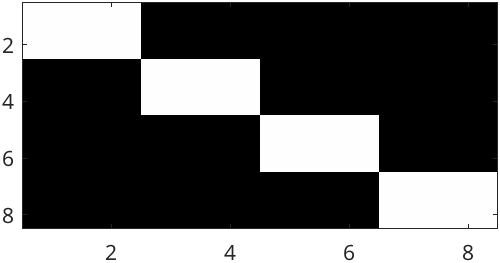
\includegraphics[width=\textwidth]{2B_Input2}
    	\caption{JPEG Input 2}
    	\label{fig:2B_Input2}
  	\end{minipage}
	\end{figure}

	\begin{figure}[ht]
  	\centering
  	\begin{minipage}[t]{0.45\textwidth}
    	\centering
    	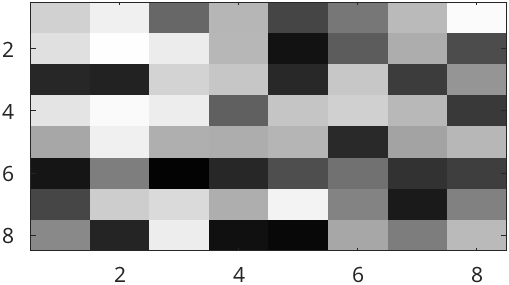
\includegraphics[width=\textwidth]{2B_Decom1}
    	\caption{Decompressed Input 1}
    	\label{fig:2B_Decom1}
  	\end{minipage}\hfill
  	\begin{minipage}[t]{0.45\textwidth}
    	\centering
    	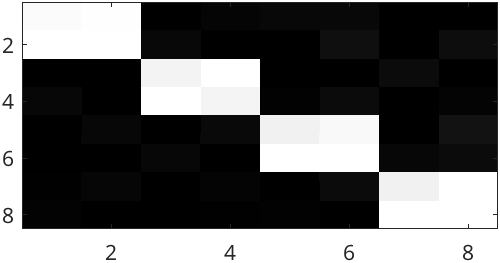
\includegraphics[width=\textwidth]{2B_Decom2}
    	\caption{Decompressed Input 2}
    	\label{fig:2B_Decom2}
  	\end{minipage}
	\end{figure}

	
	\begin{figure}[ht]
  	\centering
  	\begin{minipage}[t]{0.45\textwidth}
    	\centering
    	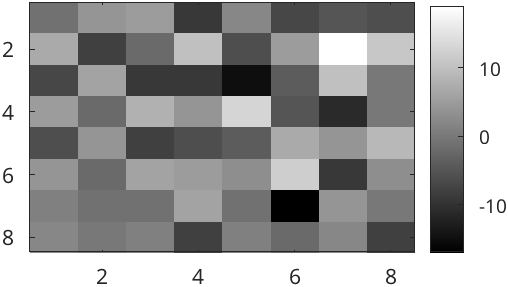
\includegraphics[width=\textwidth]{2B_Diff1}
    	\caption{Input 1 Difference (rms 8.02)}
    	\label{fig:2B_Diff1}
  	\end{minipage}\hfill
  	\begin{minipage}[t]{0.45\textwidth}
    	\centering
    	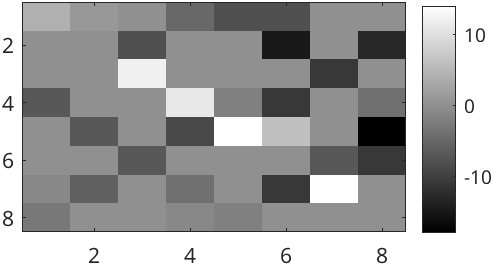
\includegraphics[width=\textwidth]{2B_Diff2}
    	\caption{Input 2 Difference (rms 6.24)}
    	\label{fig:2B_Diff2}
  	\end{minipage}
	\end{figure}

	Continuing on to the next test, we are subjected into testing the {\texttt{Q}} value first before testing the {\texttt{tolerance}} level. The test values used for {\texttt{Q}} are 
	{\texttt{1}}, {\texttt{25}}, {\texttt{50}}, {\texttt{80}}, and {\texttt{99}}. We will be using {Figure~\ref{fig:2B_Input1any}} and {Figure~\ref{fig:2B_Input1anyref}} as the input and reference 
	images for all the test	cases, respectively, unless stated. By examining {Figure~\ref{fig:2B_Input1TD}} and {Figure~\ref{fig:2B_Input5TD}}, we can observe that the quality of the image frame 
	is controlled by the parameter {\texttt{Q}}. A higher value of {\texttt{Q}} corresponds to higher image quality, while a lower value of {\texttt{Q}} corresponds to lower image quality. 
	It is evident from {Figure~\ref{fig:2B_Tolerance50}} that using a tolerance level of {\texttt{50.0}} results in disoriented pixels or artifacts. However, when the tolerance level is lowered, 
	as shown in	{Figure~\ref{fig:2B_Tolerance5}}, the image appears cleaner and clearer.

	\begin{figure}[ht]
		\centering
		\begin{subfigure}[t]{0.45\textwidth}
			\centering

			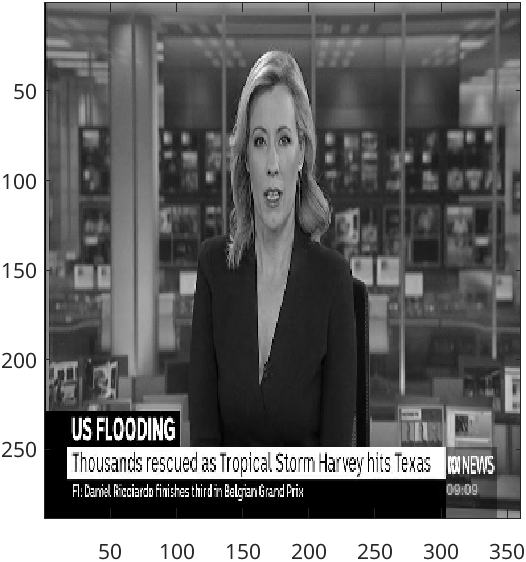
\includegraphics[width=\textwidth]{2B_Input1Orig}

			\caption{Input  1 (103680 bytes total)}
			\label{fig:2B_Input1any}

		\end{subfigure}
		\hspace{1cm}
		\begin{subfigure}[t]{0.45\textwidth}
			\centering

			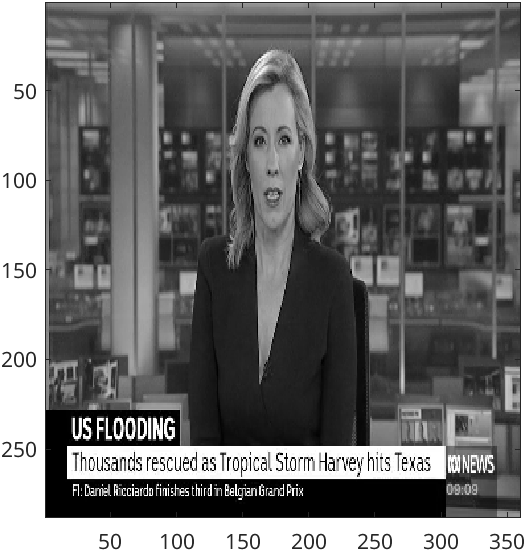
\includegraphics[width=\textwidth]{2B_Input1Ref}

			\caption{Reference}
			\label{fig:2B_Input1anyref}

		\end{subfigure}


		\caption{Input 1 at any Q and Tolerance values}
		\label{fig:2B_Input1anyall}
	\end{figure}

	\begin{figure}[ht]
		% q = 1
		\centering
		\begin{subfigure}[t]{0.45\textwidth}
			\centering

			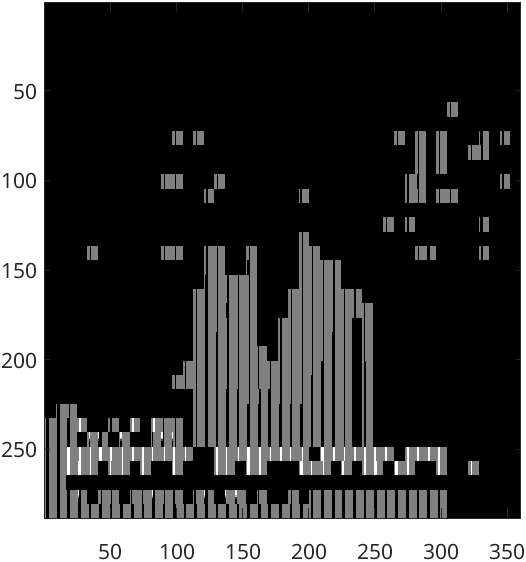
\includegraphics[width=\textwidth]{2B_Input1TD}

			\caption{Transmitted Data (516 bytes)}
			\label{fig:2B_Input1TD}

		\end{subfigure}
		\hspace{1cm}
		\begin{subfigure}[t]{0.45\textwidth}
			\centering

			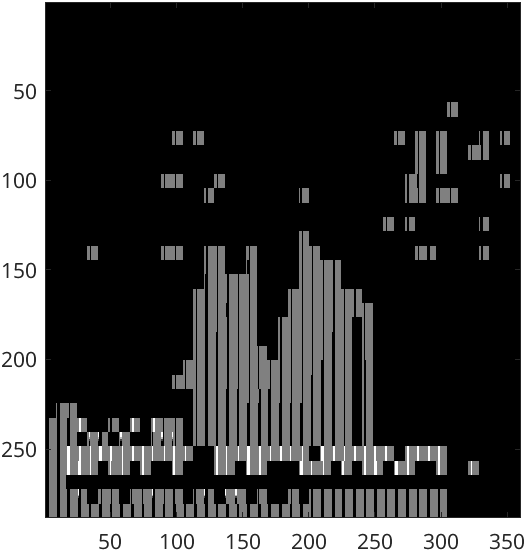
\includegraphics[width=\textwidth]{2B_Input1Reconstructed}

			\caption{Reconstructed (516 bytes total)}
			\label{fig:2B_Input1Reconstructed}

		\end{subfigure}

		\caption{Q = 1, Tolerance = 5.00}
		\label{fig:2B_Input1}
	\end{figure}

	\begin{figure}[ht]
		% new figure
		\centering
			\begin{subfigure}[t]{0.45\textwidth}
			\centering

			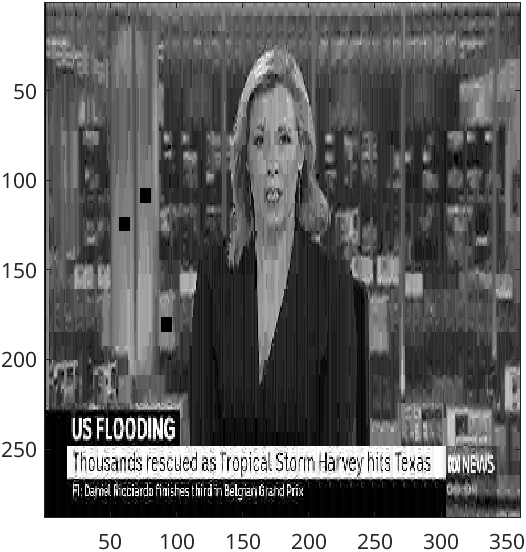
\includegraphics[width=\textwidth]{2B_Input2TD}

			\caption{Transmitted Data (15729 bytes)}
			\label{fig:2B_Input2TD}

		\end{subfigure}
		\hspace{1cm}
		\begin{subfigure}[t]{0.45\textwidth}
			\centering

			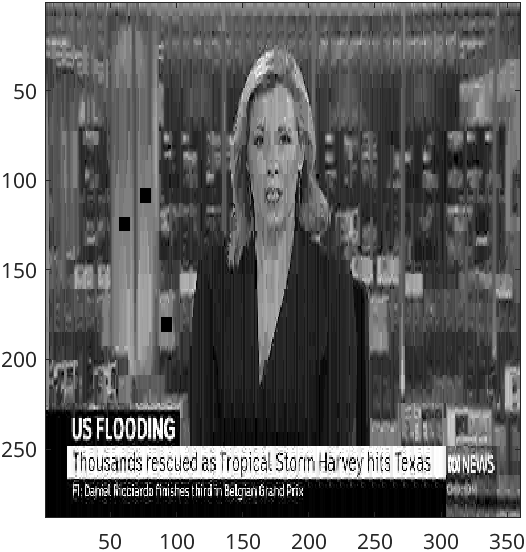
\includegraphics[width=\textwidth]{2B_Input2Reconstructed}

			\caption{Reconstructed (15729 bytes total)}
			\label{fig:2B_Input2Reconstructed}

		\end{subfigure}

		\caption{Q = 25, Tolerance = 5.00}
		\label{fig:2B_Input2}
	\end{figure}

		\begin{figure}[ht]
			% new fig
		\centering
			\begin{subfigure}[t]{0.45\textwidth}
			\centering

			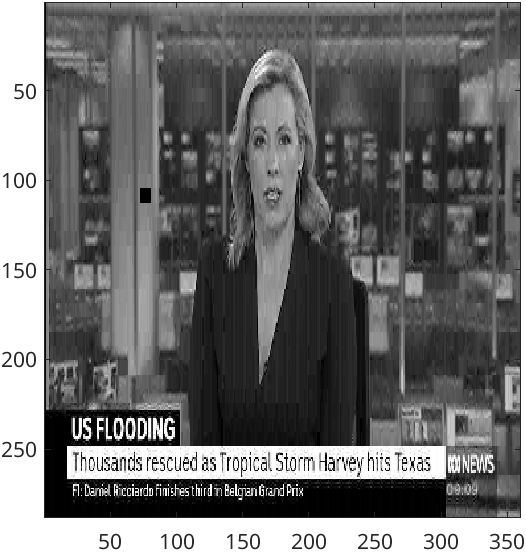
\includegraphics[width=\textwidth]{2B_Input3TD}

			\caption{Transmitted Data (21862 bytes)}
			\label{fig:2B_Input3TD}

		\end{subfigure}
		\hspace{1cm}
		\begin{subfigure}[t]{0.45\textwidth}
			\centering

			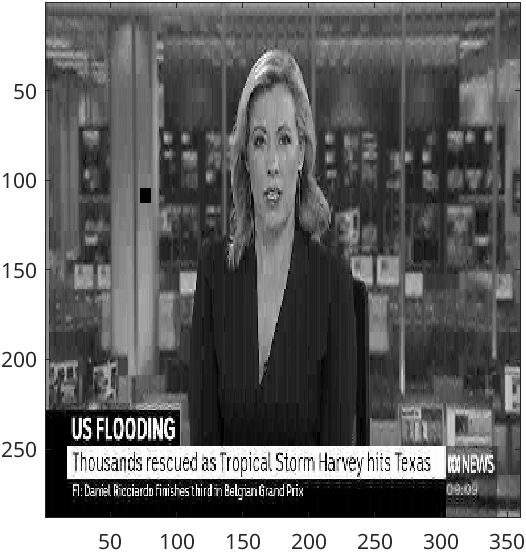
\includegraphics[width=\textwidth]{2B_Input3Reconstructed}

			\caption{Reconstructed (21862 bytes total)}
			\label{fig:2B_Input3Reconstructed}

		\end{subfigure}

		\caption{Q = 50, Tolerance = 5.00}
		\label{fig:2B_Input3}
	\end{figure}



		\begin{figure}[ht]
			% q = 80
		\centering
			\begin{subfigure}[t]{0.45\textwidth}
			\centering

			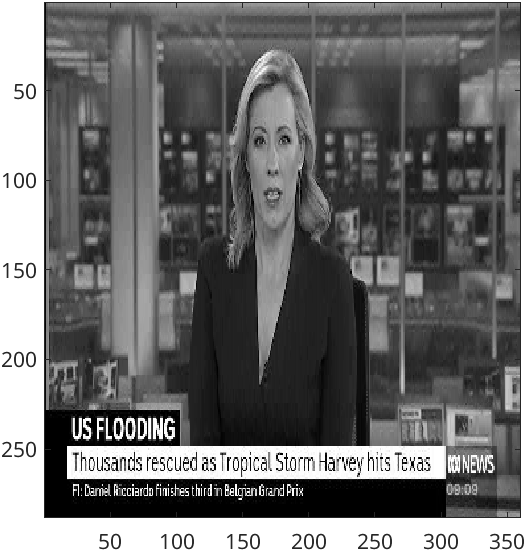
\includegraphics[width=\textwidth]{2B_Input4TD}

			\caption{Transmitted Data (31383 bytes)}
			\label{fig:2B_Input4TD}

		\end{subfigure}
		\hspace{1cm}
		\begin{subfigure}[t]{0.45\textwidth}
			\centering

			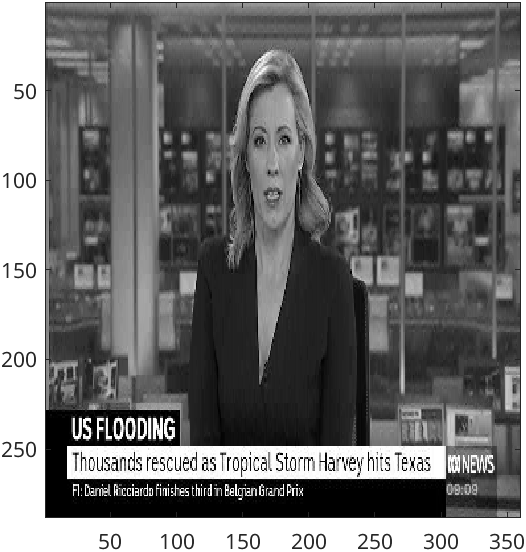
\includegraphics[width=\textwidth]{2B_Input4Reconstructed}

			\caption{Reconstructed (31383 bytes total)}
			\label{fig:2B_Input4Reconstructed}

		\end{subfigure}

		\caption{Q = 80, Tolerance = 5.00}
		\label{fig:2B_Input4}
	\end{figure}


		\begin{figure}[ht]
			% Q = 99
		\centering
			\begin{subfigure}[t]{0.45\textwidth}
			\centering

			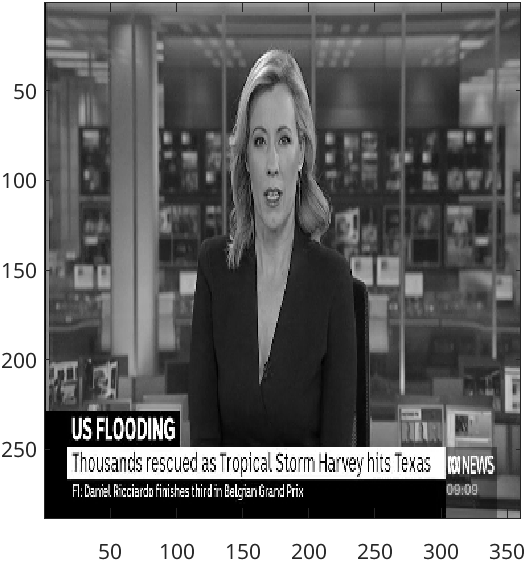
\includegraphics[width=\textwidth]{2B_Input5TD}

			\caption{Transmitted Data (83173 bytes)}
			\label{fig:2B_Input5TD}

		\end{subfigure}
		\hspace{1cm}
		\begin{subfigure}[t]{0.45\textwidth}
			\centering

			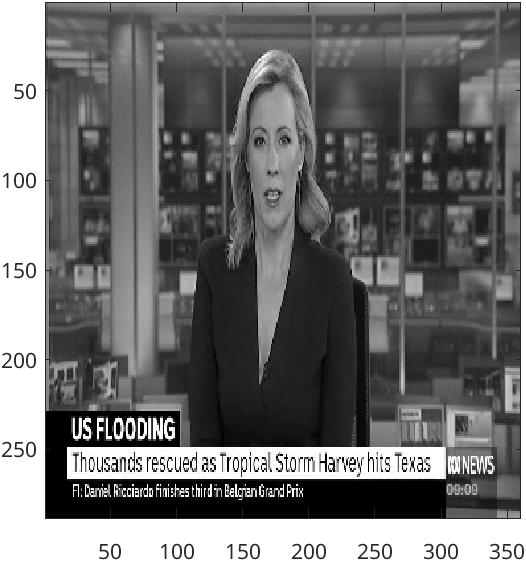
\includegraphics[width=\textwidth]{2B_Input5Reconstructed}

			\caption{Reconstructed (83173 bytes total)}
			\label{fig:2B_Input5Reconstructed}

		\end{subfigure}

		\caption{Q = 99, Tolerance = 5.00}
		\label{fig:2B_Input5}
	\end{figure}
		\begin{figure}[ht]
			% q = 80, input 8
		\centering

		\begin{subfigure}[t]{0.45\textwidth}
			\centering

			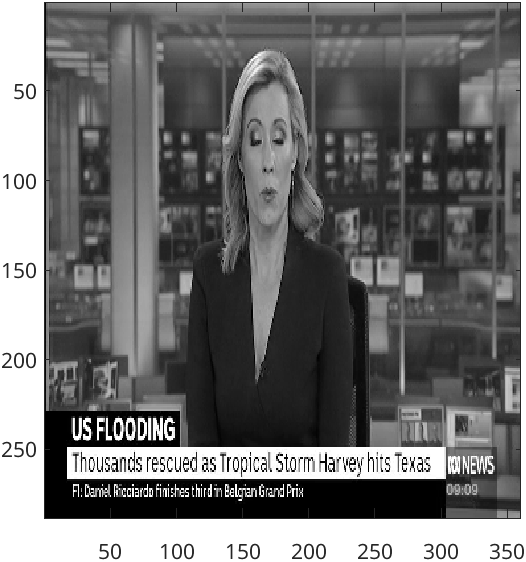
\includegraphics[width=\textwidth]{2B_Input4Orig2}

			\caption{Frame 8}
			\label{fig:2B_Input4Orig2}

		\end{subfigure}
		\hspace{1cm}
		\begin{subfigure}[t]{0.45\textwidth}
			\centering

			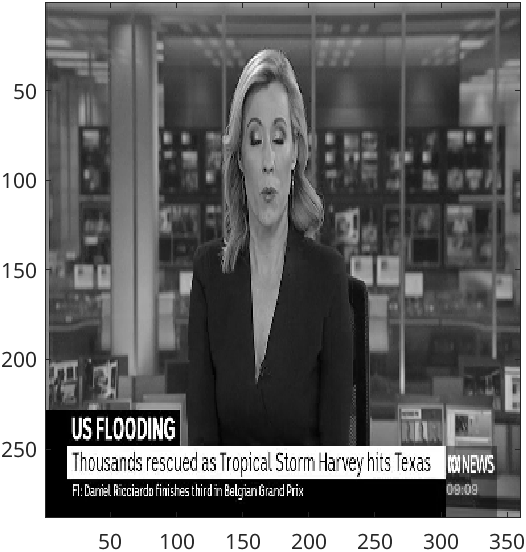
\includegraphics[width=\textwidth]{2B_Input4Ref2}

			\caption{Reference}
			\label{fig:2B_Input4Ref2}

		\end{subfigure}


			\begin{subfigure}[t]{0.45\textwidth}
			\centering

			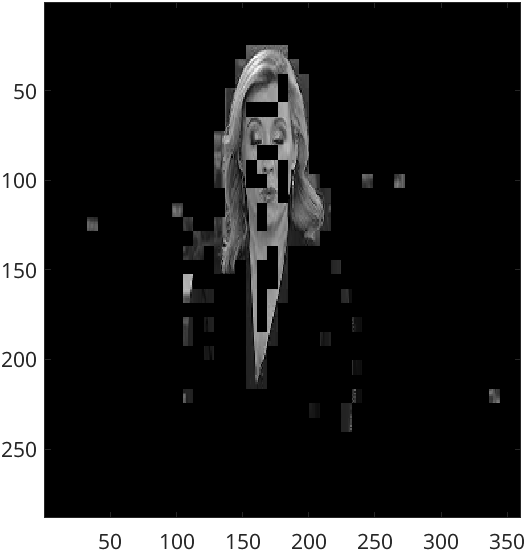
\includegraphics[width=\textwidth]{2B_Input4TD2}

			\caption{Transmitted Data (3674 bytes)}
			\label{fig:2B_Input4TD2}

		\end{subfigure}
		\hspace{1cm}
		\begin{subfigure}[t]{0.45\textwidth}
			\centering

			\includegraphics[width=\textwidth]{2B_Input4Reconstructed2}

			\caption{Reconstructed (58437 bytes total)}
			\label{fig:2B_Input4Reconstructed2}

		\end{subfigure}

		\caption{Q = 80, Tolerance = 5.00}
		\label{fig:2B_Input4b}
	\end{figure}


		\begin{figure}[ht]
			% input 100; Q = 80, tolerance = 5
		\centering
			\begin{subfigure}[t]{0.45\textwidth}
			\centering

			\includegraphics[width=\textwidth]{2B_Tolerance5Input}

			\caption{Input 100 (10368000 bytes total)}
			\label{fig:2B_Tolerance5Input}

		\end{subfigure}

			\begin{subfigure}[t]{0.45\textwidth}
			\centering

			\includegraphics[width=\textwidth]{2B_Tolerance5TD}

			\caption{Transmitted Data (2843 bytes)}
			\label{fig:2B_Tolerance5TD}

		\end{subfigure}
		\hspace{1cm}
		\begin{subfigure}[t]{0.45\textwidth}
			\centering

			\includegraphics[width=\textwidth]{2B_Tolerance5Reconstructed}

			\caption{Reconstructed (552853 bytes total)}
			\label{fig:2B_Tolerance5Reconstructed}

		\end{subfigure}

		\caption{Q = 80, Tolerance = 5.00}
		\label{fig:2B_Tolerance5}
	\end{figure}


		\begin{figure}[ht]
			% input 100; Q = 80, tolerance = 50
		\centering
			\begin{subfigure}[t]{0.45\textwidth}
			\centering

			\includegraphics[width=\textwidth]{2B_Tolerance50Input}

			\caption{Input 100 (10368000 bytes total)}
			\label{fig:2B_Tolerance50Input}

		\end{subfigure}

			\begin{subfigure}[t]{0.45\textwidth}
			\centering

			\includegraphics[width=\textwidth]{2B_Tolerance50TD}

			\caption{Transmitted Data (638 bytes)}
			\label{fig:2B_Tolerance50TD}

		\end{subfigure}
		\hspace{1cm}
		\begin{subfigure}[t]{0.45\textwidth}
			\centering

			\includegraphics[width=\textwidth]{2B_Tolerance50Reconstructed}

			\caption{Reconstructed (347376 bytes total)}
			\label{fig:2B_Tolerance50Reconstructed}

		\end{subfigure}

		\caption{Q = 80, Tolerance = 50.00}
		\label{fig:2B_Tolerance50}
	\end{figure}

	In summary, the parameter Q in the code determines the quality factor for image encoding. A higher value of Q leads to lower compression, preserving more image details and resulting in 
	higher image quality. Conversely, a lower value of Q increases compression, sacrificing some image details for higher efficiency. However, when the transmitted data gets reconstructed 
	the image data or details are lost. The tolerance level, on the other hand, determines the level of change or difference between consecutive frames that will be considered significant 
	enough to encode and transmit which is why having lower tolerance value would compress smaller compared to having high tolerance value which compresses huge data. Having a higher tolerance
	value would result image artifacts with deformed pixels.


	\subsection*{4. Comments and Conclusion}

	The completion of the {\texttt{djpeg\_8x8.m}} and {\texttt{simple\_dmpeg.m}} functions enables the decoding of JPEG images and MPEG videos, respectively. The decoding process involves quantization, inverse quantization, 
	IDCT, and comparison of frames. The experiments conducted using different parameter configurations demonstrated the influence of the {\texttt{Q}} value and tolerance level on image quality and compression efficiency. A 
	higher {\texttt{Q}} value resulted in higher image quality with less compression, while a lower {\texttt{Q}} value sacrificed image details for better compression efficiency. Lower tolerance levels produced cleaner 
	images with fewer artifacts, while higher tolerance levels resulted in more noticeable artifacts.

	These findings emphasize the importance of choosing appropriate parameter values in image and video decoding to balance the trade-off between image quality and compression efficiency. The completed functions provide 
	a foundation for further research and development in the field of image and video processing.




	
	\vspace{0.5cm}
	\clearpage
	\newpage
	\section*{Exercise 2C -- (2\%) -- Written Questions }
	

	\begin{itemize}
		\item{\textbf{2C.1} (0.5\%)}
			{
				\begin{itemize}
					\item[A.] 
						Considering the absence of lens distortion, the optimal transformation to capture the relationship between images in this situation is a projective linear transformation. This type of transformation is 
						particularly suited for scenarios where points in an image plane need to be mapped to points in a 3D space, and vice versa. It enables the projection of 3D points onto the 2D image plane, as illustrated in 
						the lecture material on spatial transformations. When it comes to celestial objects like Jupiter, the projective linear transformation is an ideal choice for 
						capturing their projection onto a 2D image plane. The camera records the celestial body's appearance in a 2D format, with the transformation preserving the relative positions and shapes 
						of objects within the scene.

						When the telescope is adjusted or moved, it captures different views of the celestial body, altering the perspective of the scene being recorded by the camera. Each change in 
						perspective results in a unique mapping of the 3D scene onto the 2D image plane. Consequently, the captured image presents a specific viewpoint of the camera, showcasing the celestial body from a 
						particular vantage point.

					\item[B.]
						In the given scenario, where the transformation of the document itself is the focus rather than the room, the most appropriate transformation would be an {\texttt{affine linear transformation}}. 
						This choice is based on the requirement to maintain the document's proportions and parallelism when it is photographed and viewed from different angles and positions. Other linear transformations 
						are not suitable for this situation. Like for example, projective transformation, not preserve parallel lines and involves planar scaling, which is not applicable in this case where the document 
						is observed from various positions within the room. Isometry, another type of transformation, preserves distances, but it is not feasible in this context as the observer moves to different locations in the room. 
						Linear-conformal transformation, which preserves shape, is also unsuitable as the picture may be taken from different angles, resulting in a change in shape. Translation, which is a simple rigid transformation 
						involving movement, is not relevant here since the viewpoint remains fixed.

						Therefore, the {\texttt{affine linear transformation}} stands out as the most appropriate choice for maintaining the document's proportions and parallelism while allowing for variations in viewing angles and positions. 
						This makes sure that the document appears consistent and accurately represents its original geometry despite changes in perspective.

				\end{itemize}
			}
		
		\item{\textbf{2C.2} (0.5\%)}
			
						Given the matrix transformation of linear-conformal, we equate the given matrix representation of the linear transformation and then solve for the values.

						$
							T = \begin{bmatrix}
  									sR_2 & t \\
  									0 & 1
									\end{bmatrix}
								= \begin{bmatrix}
									s(\cos(\theta))  & s(\sin(\theta)) & t_x \\
									s(-\sin(\theta)) & s(\cos(\theta)) & t_y \\
									0 & 0 & 1
									\end{bmatrix}
								= \begin{bmatrix}
									1.7321 	& 1 		  & 10 	\\
									-1 		  & -1.7321	& -20 \\
									0       & 0       & 1
								\end{bmatrix}
						$

						Then we have these system of equations:

						$t_x = 10$; $t_y = -20$; $s(\cos(\theta)) = 1.7321$; $s(\sin(\theta)) = 1$

						Solving for the rotation:

						$s = \frac{1.7321}{\cos\theta}$; $s = \frac{1}{\sin\theta}$

						Equating those into:
						
						\begin{align*}
							\frac{1.7321}{\cos\theta}\sin\theta & = 1 \\
							1.7321\tan\theta                    & = 1 \\
							\tan\theta                          & = \frac{1}{1.7321} \\
							\theta                              & = \arctan({\frac{1}{1.7321})} \\
							\theta                              & = 30^{\circ}
						\end{align*}

						Using the $\theta$ value we acquired, we can now get the scale value:


						\begin{align*}
							s & = \frac{1.7321}{cos\theta} \\
							s & = \frac{1.7321}{cos(30^{\circ})} \\
							s & \approx 2.000056803 = 2
						\end{align*}

						Thus, our translation values are:

						
						\begin{align*}
							t_x    & = 10 \\
							t_y    & = -20 \\
							\theta & = 30^{\circ} \\
							s & = 2
						\end{align*}


		\item{\textbf{2C.3} (0.5\%)}


			We will use {Equation~\ref{eq:BilinearInterpolationFormula}} for the bilinear interpolation:
			\begin{equation}
				\begin{split}
    				I(p) &= [(1-a)(1-b)(I(x,y))] \\
    				&\quad+ [(1-a)(b)(I(x,y+1))] \\
    				&\quad+ [(a)(1-b)(I(x+1,y))] \\
    				&\quad+ [(a)(b)(I(x+1,y+1))]
				\end{split}
				\label{eq:BilinearInterpolationFormula}
			\end{equation}
			In order to get the values $a$ and $b$ for the bilinear estimates for pixel (20.6, 10.2), we can use {Equation~\ref{eq:BIa}} and {Equation~\ref{eq:BIb}}:

			\begin{equation}
				\begin{split}
				  a & = p_x - \lfloor p_x \rfloor \\
				   & = 20.6 - \lfloor 20.6 \rfloor \\
				   & = 20.6 - 20 \\
				  a & = 0.6
				\end{split}
				\label{eq:BIa}
			\end{equation}
			\begin{equation}
				\begin{split}
				  b & = p_y - \lfloor p_y \rfloor \\
				   & = 10.2 - \lfloor 10.2 \rfloor \\
				   & = 10.2 - 10 \\
				  b & = 0.2
				\end{split}
				\label{eq:BIb}
			\end{equation}

			Now that $a$ and $b$ values have been determined, we can substitute those values into Equation~\ref{eq:BilinearInterpolationFormula}. Thus, we get {Equation~\ref{eq:BISolution}}:

			\begin{equation}
				\begin{split}
    				I(p) &= [(1-0.6)(1-0.2)(128)] + [(1-0.6)(0.2)(64)] + [(0.6)(1-0.2)(64)] \\
    				&\quad+ [(0.6)(0.2)(32)] \\
    				&=      [(0.4)(0.8)(128)] + [(0.4)(0.2)(64)] + [(0.6)(0.8)(64)] + [(0.6)(0.2)(32)] \\
    				&=      40.96 + 5.12 + 30.72 + 3.84 \\ 
    				I(p) &= 80.64
				\end{split}
				\label{eq:BISolution}
			\end{equation}

			Thus, the bilinear estimate for the pixel $(20.6, 10.2)$ is {\texttt{80.64}} and its nearest neighbor is $(21,10)$ shown on {Figure~\ref{fig:2CGraph}}. However, if we follow the formula

			\begin{figure}
  			\centering
  			\includegraphics[width=0.5\textwidth]{2CGraph}
  			\caption{Nearest neighboring pixels of (20.6, 10.2)}
  			\label{fig:2CGraph}
			\end{figure}

		\item{\textbf{2C.4} (0.5\%)}

			Based on a detailed analysis of the spectral characteristics and their corresponding outputs, we can draw specific conclusions regarding the relationship between {\texttt{Spectra 1}}, 
			{\texttt{Spectra 2}}, and their respective outputs.

			Firstly, {\texttt{Spectra 1}} can be attributed to the generation of {\texttt{Output 2}} due to its distinctive composition of black and white. This composition is reflected in the 
			resulting image, where the cameraman is prominently highlighted in white against a mostly black background with subtle gray shades. The presence of blacks and whites in {\texttt{Spectra 1}} 
			contributes to the stark contrast between the subject and the background, emphasizing the cameraman's features. Notice that {\texttt{Spectra 1}} shows a relatively smoother profile without 
			any prominent stripes, implying a more uniform background. This aligns with the characteristics of {\texttt{Output 1}}, which exhibits a consistent and evenly distributed response

			As for {\texttt{Spectra 2}}, it is found to be responsible for the creation of {\texttt{Output 1}}. This conclusion is supported by the predominantly gray background observed in the 
			resulting image. The grayscale background, with a central black line indicating the presence of dark edges around objects, aligns with the spectral characteristics of {\texttt{Spectra 2}}. 
			The absence of distinct black and white regions suggests a more uniform distribution of gray tones, resulting in a less contrasting image.

	\end{itemize}
	


\end{document}
